
\newcommand{\FigOverview}{
\begin{figure}[ht]
    \centering
    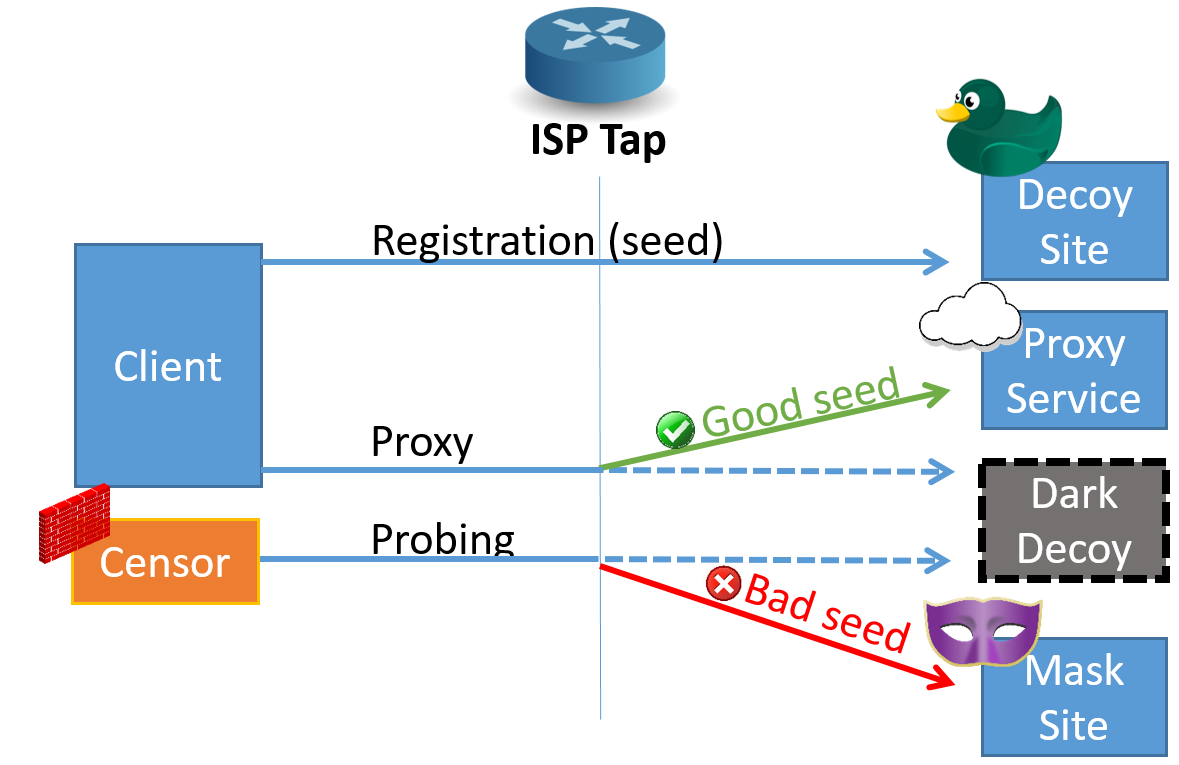
\includegraphics[width=0.9\linewidth,clip]{figures/dark-decoy-overview.png}
    \caption{\textbf{Dark Decoy Overview}\,---\, %
    }
    \label{fig:overview}
\end{figure}
}

\newcommand{\FigHighLevel}{
\begin{figure}[t]
    \centering
    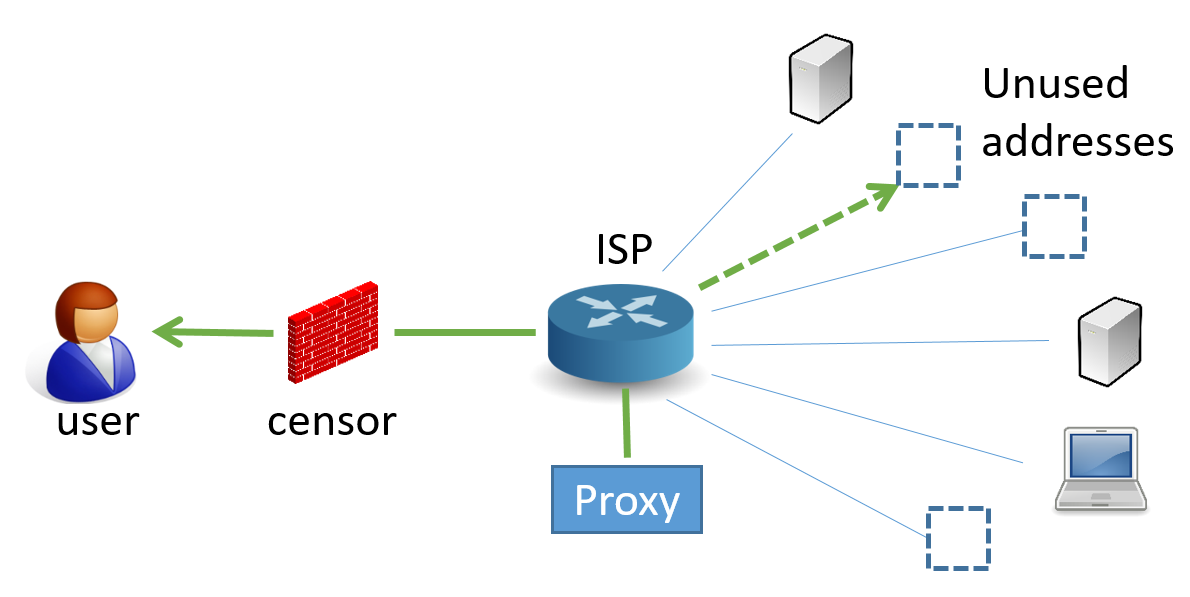
\includegraphics[width=0.9\linewidth,clip]{figures/high-level.png}
    \caption{\textbf{Dark Decoys}\,---\, %
    After registering, clients connect to unused (``dark'') addresses that pass
        by a cooperating ISP proxy station. The station communicates with the client
        as if it were a host at the particular address. To the censor, this
        communication appears to be a legitimate connection to a real host,
        making it difficult to distinguish from real hosts and block.
    }
    \label{fig:overview}
\end{figure}
}

